\documentclass[11pt,a4paper,oneside]{article}

\usepackage{cmap}
\usepackage[utf8]{inputenc}
\usepackage[warn]{mathtext}
\usepackage{epsf,amsmath,amsfonts,amssymb,amsbsy}
\usepackage[mathscr]{eucal}
\usepackage[english, russian]{babel}
\usepackage[left=2cm,right=2cm,top=2cm,bottom=2cm]{geometry}
\usepackage{graphicx}
\usepackage{indentfirst}
\usepackage{pgfplots}

% running titles 
\usepackage{fancybox}
\usepackage{fancyhdr}

% for diff running titles on pages with diff parity
\usepackage{ifthen}
\usepackage{pdfpages}
\usepackage[strict]{changepage}

% page style setup (for running titles)
\fancypagestyle{plain}{ %
\fancyhf{} % remove everything

\graphicspath{{pictures2.1.3/}}
\DeclareGraphicsExtensions{.pdf,.png,.jpg}

 % lines parameters
\renewcommand{\headrulewidth}{0pt}
\renewcommand{\footrulewidth}{0pt}

% running titles contents
\fancyfoot[L]{\ifthenelse{\isodd{\thepage}}{Работа 2.1.3}{\thepage}}
\fancyfoot[R]{\ifthenelse{\isodd{\thepage}}{\thepage}{Работа 2.1.3}}
}

% choosing page style with our running titles
\pagestyle{plain}


%\title{«МОСКОВСКИЙ ФИЗИКО-ТЕХНИЧЕСКИЙ ИНСТИТУТ (НАЦИОНАЛЬНЫЙ ИССЛЕДОВАТЕЛЬСКИЙ УНИВЕРСИТЕТ)»}
\author{Матренин Василий Б01-006 ФРКТ}
\title{Отчёт о выполнении лабораторной работы 2.1.3}

\begin{document}
	\maketitle
	\begin{center}
		{\Large Определение $C_p/C_v$ по скорости звука в газе}
	\end{center}
	\paragraph*{Цель работы:} 1) измерение частоты
	колебаний
	и длины волны при
	резонансе звуковых
	колебаний в газе, заполняющем трубу; 2) определение показателя адиабаты с помощью уравнения состояния идеального газа.
	\paragraph*{В работе используются:} звуковой генератор ГЗ; электронный
	осциллограф ЭО; микрофон; телефон; раздвижная труба; теплоизолированная труба, обогреваемая водой из термостата; баллон
	со сжатым углекислым газом; газгольдер.
	\section{Теоретическое введение}
	
		Cкорость распространения звуковой волны в газах зависит от показателя адиабаты $\gamma$. На измерении скорости звука основан один из наиболее  точных методов определения показателя  адиабаты.
		
		Скорость звука в газах определяется формулой:
		$$c=\sqrt{\gamma\frac{RT}{\mu}},$$
		где $R$ - газовая постоянная, $T$ - температура газа, а $\mu$ его молярная масса. Выразим показатель адиабаты:
		$$\gamma=\frac{\mu}{RT} c^2$$
		
		Звуковая волна, распространяющаяся вдоль трубы, испытывает многократные отражения от торцов. Звуковые колебания в трубе являются наложением всех отраженных волн и, вообще говоря, очень сложны. Картина упрощается, если длина трубы L равна целому числу полуволн, то есть когда
		$$L=n\frac{\lambda}{2},$$
		где $\lambda$ — длина волны звука в трубе, а $n$ — любое целое число.
		
		Скорость звука c связана с его частотой $f$ и длиной волны $\lambda$ соотношением:
		$$c=\lambda f.$$
		
		Подбор условий, при которых возникает резонанс, можно производить двояко:
		
		1) При неизменной частоте f звукового генератора (а следовательно, и неизменной длине звуковой волны $\lambda$) можно изменять длину трубы $L$. Для этого применяется раздвижная труба. Длина раздвижной трубы постепенно увеличивается, и наблюдается ряд последовательных резонансов. Для $k$-ого резонанса имеем:
		$$L_{n+k}=n\frac{\lambda}{2} + k\frac{\lambda}{2},$$
		т. е. $\lambda/2$ равно угловому коэффициенту графика, изображающего зависимость длины трубы $L$ от номера резонанса $k$.
		
		2) При постоянной длине трубы можно изменять частоту звуковых
		колебаний. В этом случае следует плавно изменять частоту $f$ звукового генератора, а следовательно, и длину звуковой волны $\lambda$.
		Для $k$-ого резонанса получим:

		$$L = (n+k)\frac{\lambda_{k+1}}{2}$$
		$$f_{k+1} = \frac{c}{\lambda_{k+1}}=\frac{c}{2L}(n+k)=f_1 + \frac{c}{2L}k.$$
		
		Скорость звука, деленная на $2L$, определяется, таким образом,
		по угловому коэффициенту графика зависимости частоты от номера
		резонанса.
	\subsection{Эксперементальная установка:}
	\begin{figure}[h]
	\center{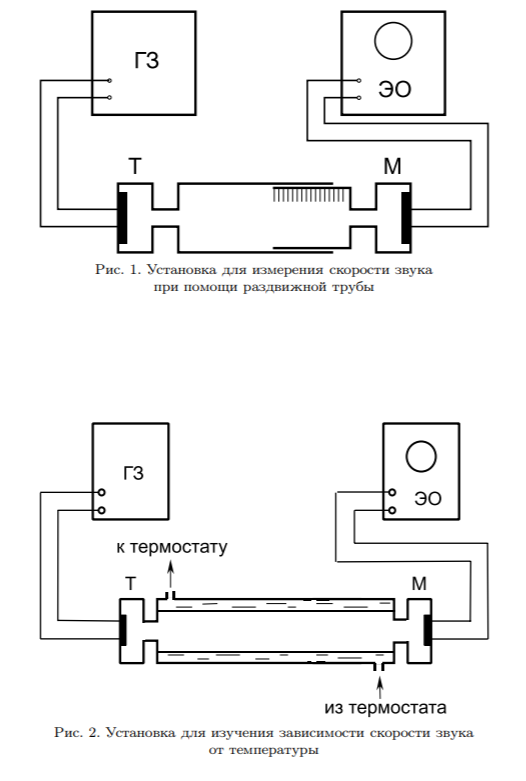
\includegraphics[scale=0.65]{lab_2_1_3_ust}}
	\end{figure}
	Соответственно двум методам измерения скорости звука в работе имеются две установки (рис. 1 и 2). В обеих установках звуковые колебания в трубе возбуждаются телефоном Т и улавливаются микрофоном М. Мембрана телефона приводится в движение переменным током звуковой частоты; в качестве источника переменной ЭДС используется звуковой генератор ГЗ. Возникающий в микрофоне сигнал наблюдается на осциллографе ЭО.

	Микрофон и телефон присоединены к установке через тонкие резиновые трубки. Такая связь достаточна для возбуждения и обнаружения звуковых колебаний в трубе и в то же время мало возмущает эти колебания: при расчетах оба торца трубы можно считать неподвижными, а влиянием соединительных отверстий пренебречь.

	Первая установка (рис. 1) содержит раздвижную трубу с миллиметровой шкалой. Через патрубок (на рисунке не показан) труба может наполняться воздухом или углекислым газом из газгольдера. На этой установке производятся измерения $\gamma$ для воздуха и для $CO_2$.
	
	Вторая установка (рис. 2) содержит теплоизолированную трубу постоянной длины. Воздух в трубе нагревается водой из термостата. Температура газа принимается равной температуре омывающей трубу воды. На этой установке измеряется зависимость скорости звука от температуры.

	\newpage

	\subsection{Ход работы}
	\begin{enumerate}
		\item Перепишем параметры установки:
		$L = 570\pm1 \; {мм}.$
		\item  
		
		Исходя из примерного значения скорости звука ($ \approx 270 \; \frac{м}{с}$), предварительно рассчитаем, в каком диапазоне частот следует вести измерения, чтобы при удлинении трубы можно было наблюдать 4 резонанса:
		$L = \frac{n\lambda}{2}$, $L + \Delta L = \frac{(n+4)\lambda}{2}$. Поскольку $\Delta L \leq 23 \; {см}$, то $\lambda \leq 11.5 \; {см}$. Следовательно $f \geq 2400 \; {гц}. $
		
		Проведём измерения на первой установке для воздуха и $CO_2$.
		Плавно изменяя длину трубы, последовательно зафиксируем все доступные для наблюдения точки резонанса. Измерения проводятся для нескольких частот.
		Занесем данные в таблицу 1.

\item Изобразим полученные результаты на графике, откладывая по оси абсцисс номер $k$ последовательного резонанса, а по оси ординат — соответствующее удлинение трубы
$L$. Угловой коэффициент прямой определяет длину полуволны.
		
Построим график 1: зависимости удлинения L от номера резонанса k \textbf{для воздуха}.

\begin{figure}[h!]
    \centering
	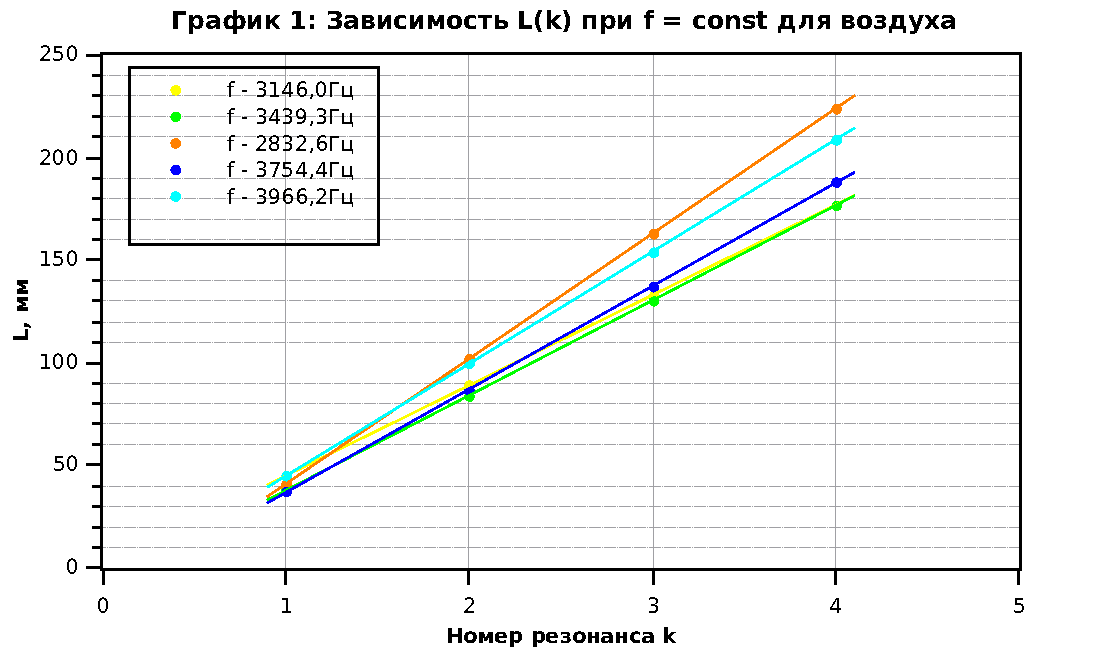
\includegraphics[scale=0.8]{Graph1.pdf}
	
\end{figure} 
\newpage
Также построим график 2: зависимости удлинения L от номера резонанса k \textbf{для углекислого газа}.
\begin{figure}[h!]
\centering
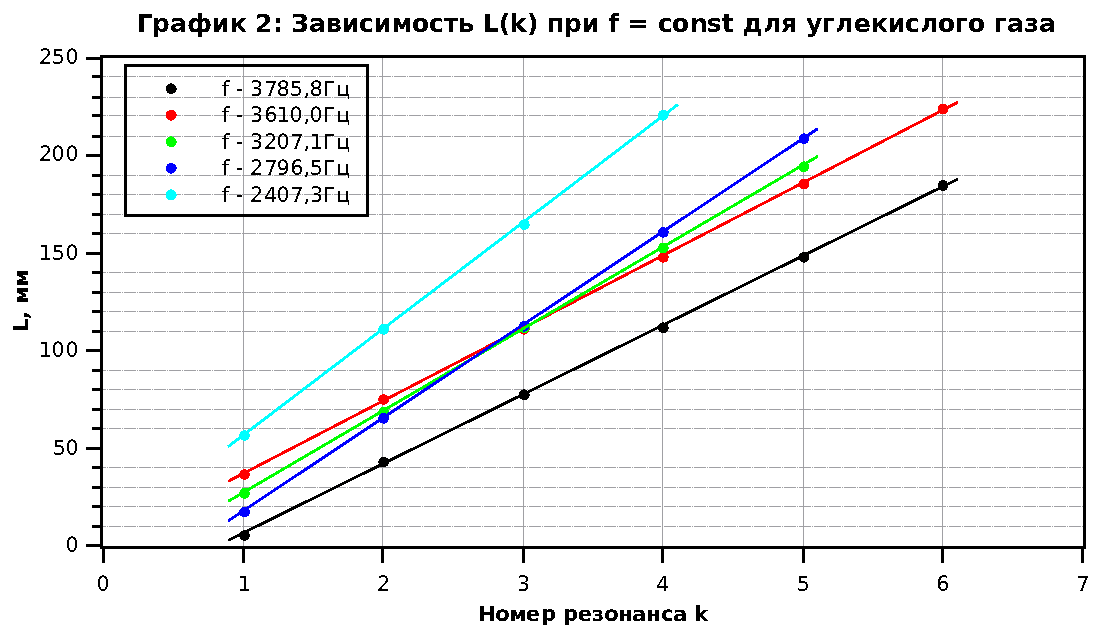
\includegraphics[scale=0.8]{Graph2.pdf}
\end{figure} 


\begin{center}
\begin{table}[h!]
\begin{tabular}{ccccccccccc}
\multicolumn{11}{c}{\textbf{Таблица 1. Зависимость L(k) для воздуха и CO2}}                                                                                                                                                                                                                                                                                                                                                    \\ \hline
\multicolumn{5}{|c|}{\textbf{Воздух}}                                                                                                                                                          & \multicolumn{1}{c|}{}          & \multicolumn{5}{c|}{\textbf{CO2}}                                                                                                                                                             \\ \hline
\multicolumn{1}{|c|}{\textbf{k}} & \multicolumn{1}{c|}{\textbf{f, Гц}} & \multicolumn{1}{c|}{\textbf{L, мм}} & \multicolumn{1}{c|}{\textbf{$\Delta$L, мм}}  & \multicolumn{1}{c|}{\textbf{с, м/c}} & \multicolumn{1}{c|}{\textbf{}} & \multicolumn{1}{c|}{\textbf{k}} & \multicolumn{1}{c|}{\textbf{f, Гц}} & \multicolumn{1}{c|}{\textbf{L, мм}} & \multicolumn{1}{c|}{\textbf{$\Delta$L, мм}} & \multicolumn{1}{c|}{\textbf{с, м/c}} \\ \hline
\multicolumn{1}{|c|}{1}          & \multicolumn{1}{c|}{3146,0}         & \multicolumn{1}{c|}{45}             & \multicolumn{1}{c|}{---}                     & \multicolumn{1}{c|}{---}             & \multicolumn{1}{c|}{}          & \multicolumn{1}{c|}{1}          & \multicolumn{1}{c|}{2407,3}         & \multicolumn{1}{c|}{57}             & \multicolumn{1}{c|}{---}                    & \multicolumn{1}{c|}{---}             \\ \hline
\multicolumn{1}{|c|}{2}          & \multicolumn{1}{c|}{3146,0}         & \multicolumn{1}{c|}{100}            & \multicolumn{1}{c|}{55}                      & \multicolumn{1}{c|}{342,91}          & \multicolumn{1}{c|}{}          & \multicolumn{1}{c|}{2}          & \multicolumn{1}{c|}{2407,3}         & \multicolumn{1}{c|}{111}            & \multicolumn{1}{c|}{54}                     & \multicolumn{1}{c|}{259,99}          \\ \hline
\multicolumn{1}{|c|}{3}          & \multicolumn{1}{c|}{3146,0}         & \multicolumn{1}{c|}{154}            & \multicolumn{1}{c|}{55}                      & \multicolumn{1}{c|}{342,91}          & \multicolumn{1}{c|}{}          & \multicolumn{1}{c|}{3}          & \multicolumn{1}{c|}{2407,3}         & \multicolumn{1}{c|}{165}            & \multicolumn{1}{c|}{54}                     & \multicolumn{1}{c|}{259,99}          \\ \hline
\multicolumn{1}{|c|}{4}          & \multicolumn{1}{c|}{3146,0}         & \multicolumn{1}{c|}{209}            & \multicolumn{1}{c|}{55}                      & \multicolumn{1}{c|}{346,06}          & \multicolumn{1}{c|}{}          & \multicolumn{1}{c|}{4}          & \multicolumn{1}{c|}{2407,3}         & \multicolumn{1}{c|}{221}            & \multicolumn{1}{c|}{56}                     & \multicolumn{1}{c|}{269,62}          \\ \hline
\multicolumn{1}{|c|}{}           & \multicolumn{1}{c|}{}               & \multicolumn{1}{c|}{}               & \multicolumn{1}{c|}{}                        & \multicolumn{1}{c|}{}                & \multicolumn{1}{c|}{}          & \multicolumn{1}{c|}{}           & \multicolumn{1}{c|}{}               & \multicolumn{1}{c|}{}               & \multicolumn{1}{c|}{}                       & \multicolumn{1}{c|}{}                \\ \hline
\multicolumn{1}{|c|}{1}          & \multicolumn{1}{c|}{3439,3}         & \multicolumn{1}{c|}{37}             & \multicolumn{1}{c|}{---}                     & \multicolumn{1}{c|}{---}             & \multicolumn{1}{c|}{}          & \multicolumn{1}{c|}{1}          & \multicolumn{1}{c|}{2796,5}         & \multicolumn{1}{c|}{18}             & \multicolumn{1}{c|}{---}                    & \multicolumn{1}{c|}{---}             \\ \hline
\multicolumn{1}{|c|}{2}          & \multicolumn{1}{c|}{3439,3}         & \multicolumn{1}{c|}{87}             & \multicolumn{1}{c|}{50}                      & \multicolumn{1}{c|}{343,93}          & \multicolumn{1}{c|}{}          & \multicolumn{1}{c|}{2}          & \multicolumn{1}{c|}{2796,5}         & \multicolumn{1}{c|}{66}             & \multicolumn{1}{c|}{48}                     & \multicolumn{1}{c|}{265,67}          \\ \hline
\multicolumn{1}{|c|}{3}          & \multicolumn{1}{c|}{3439,3}         & \multicolumn{1}{c|}{137}            & \multicolumn{1}{c|}{50}                      & \multicolumn{1}{c|}{343,93}          & \multicolumn{1}{c|}{}          & \multicolumn{1}{c|}{3}          & \multicolumn{1}{c|}{2796,5}         & \multicolumn{1}{c|}{113}            & \multicolumn{1}{c|}{48}                     & \multicolumn{1}{c|}{265,67}          \\ \hline
\multicolumn{1}{|c|}{4}          & \multicolumn{1}{c|}{3439,3}         & \multicolumn{1}{c|}{188}            & \multicolumn{1}{c|}{51}                      & \multicolumn{1}{c|}{350,81}          & \multicolumn{1}{c|}{}          & \multicolumn{1}{c|}{4}          & \multicolumn{1}{c|}{2796,5}         & \multicolumn{1}{c|}{161}            & \multicolumn{1}{c|}{48}                     & \multicolumn{1}{c|}{268,46}          \\ \hline
\multicolumn{1}{|c|}{5}          & \multicolumn{1}{c|}{---}            & \multicolumn{1}{c|}{---}            & \multicolumn{1}{c|}{---}                     & \multicolumn{1}{c|}{---}             & \multicolumn{1}{c|}{}          & \multicolumn{1}{c|}{5}          & \multicolumn{1}{c|}{2796,5}         & \multicolumn{1}{c|}{209}            & \multicolumn{1}{c|}{48}                     & \multicolumn{1}{c|}{268,46}          \\ \hline
\multicolumn{1}{|c|}{}           & \multicolumn{1}{c|}{}               & \multicolumn{1}{c|}{}               & \multicolumn{1}{c|}{}                        & \multicolumn{1}{c|}{}                & \multicolumn{1}{c|}{}          & \multicolumn{1}{c|}{}           & \multicolumn{1}{c|}{}               & \multicolumn{1}{c|}{}               & \multicolumn{1}{c|}{}                       & \multicolumn{1}{c|}{}                \\ \hline
\multicolumn{1}{|c|}{1}          & \multicolumn{1}{c|}{2832,6}         & \multicolumn{1}{c|}{41}             & \multicolumn{1}{c|}{---}                     & \multicolumn{1}{c|}{---}             & \multicolumn{1}{c|}{}          & \multicolumn{1}{c|}{1}          & \multicolumn{1}{c|}{3207,0}         & \multicolumn{1}{c|}{27}             & \multicolumn{1}{c|}{---}                    & \multicolumn{1}{c|}{---}             \\ \hline
\multicolumn{1}{|c|}{2}          & \multicolumn{1}{c|}{2832,6}         & \multicolumn{1}{c|}{102}            & \multicolumn{1}{c|}{61}                      & \multicolumn{1}{c|}{345,58}          & \multicolumn{1}{c|}{}          & \multicolumn{1}{c|}{2}          & \multicolumn{1}{c|}{3207,0}         & \multicolumn{1}{c|}{69}             & \multicolumn{1}{c|}{42}                     & \multicolumn{1}{c|}{269,39}          \\ \hline
\multicolumn{1}{|c|}{3}          & \multicolumn{1}{c|}{2832,6}         & \multicolumn{1}{c|}{163}            & \multicolumn{1}{c|}{61}                      & \multicolumn{1}{c|}{345,58}          & \multicolumn{1}{c|}{}          & \multicolumn{1}{c|}{3}          & \multicolumn{1}{c|}{3207,0}         & \multicolumn{1}{c|}{112}            & \multicolumn{1}{c|}{43}                     & \multicolumn{1}{c|}{275,80}          \\ \hline
\multicolumn{1}{|c|}{4}          & \multicolumn{1}{c|}{2832,6}         & \multicolumn{1}{c|}{224}            & \multicolumn{1}{c|}{61}                      & \multicolumn{1}{c|}{345,58}          & \multicolumn{1}{c|}{}          & \multicolumn{1}{c|}{4}          & \multicolumn{1}{c|}{3207,0}         & \multicolumn{1}{c|}{153}            & \multicolumn{1}{c|}{41}                     & \multicolumn{1}{c|}{262,97}          \\ \hline
\multicolumn{1}{|c|}{5}          & \multicolumn{1}{c|}{---}            & \multicolumn{1}{c|}{---}            & \multicolumn{1}{c|}{---}                     & \multicolumn{1}{c|}{---}             & \multicolumn{1}{c|}{}          & \multicolumn{1}{c|}{5}          & \multicolumn{1}{c|}{3207,0}         & \multicolumn{1}{c|}{195}            & \multicolumn{1}{c|}{42}                     & \multicolumn{1}{c|}{269,39}          \\ \hline
\multicolumn{1}{|c|}{}           & \multicolumn{1}{c|}{}               & \multicolumn{1}{c|}{}               & \multicolumn{1}{c|}{}                        & \multicolumn{1}{c|}{}                & \multicolumn{1}{c|}{}          & \multicolumn{1}{c|}{}           & \multicolumn{1}{c|}{}               & \multicolumn{1}{c|}{}               & \multicolumn{1}{c|}{}                       & \multicolumn{1}{c|}{}                \\ \hline
\multicolumn{1}{|c|}{1}          & \multicolumn{1}{c|}{3754,4}         & \multicolumn{1}{c|}{38}             & \multicolumn{1}{c|}{---}                     & \multicolumn{1}{c|}{---}             & \multicolumn{1}{c|}{}          & \multicolumn{1}{c|}{1}          & \multicolumn{1}{c|}{3610,0}         & \multicolumn{1}{c|}{37}             & \multicolumn{1}{c|}{---}                    & \multicolumn{1}{c|}{---}             \\ \hline
\multicolumn{1}{|c|}{2}          & \multicolumn{1}{c|}{3754,4}         & \multicolumn{1}{c|}{84}             & \multicolumn{1}{c|}{46}                      & \multicolumn{1}{c|}{345,40}          & \multicolumn{1}{c|}{}          & \multicolumn{1}{c|}{2}          & \multicolumn{1}{c|}{3610,0}         & \multicolumn{1}{c|}{75}             & \multicolumn{1}{c|}{38}                     & \multicolumn{1}{c|}{274,36}          \\ \hline
\multicolumn{1}{|c|}{3}          & \multicolumn{1}{c|}{3754,4}         & \multicolumn{1}{c|}{130}            & \multicolumn{1}{c|}{46}                      & \multicolumn{1}{c|}{345,40}          & \multicolumn{1}{c|}{}          & \multicolumn{1}{c|}{3}          & \multicolumn{1}{c|}{3610,0}         & \multicolumn{1}{c|}{111}            & \multicolumn{1}{c|}{36}                     & \multicolumn{1}{c|}{259,92}          \\ \hline
\multicolumn{1}{|c|}{4}          & \multicolumn{1}{c|}{3754,4}         & \multicolumn{1}{c|}{177}            & \multicolumn{1}{c|}{47}                      & \multicolumn{1}{c|}{352,91}          & \multicolumn{1}{c|}{}          & \multicolumn{1}{c|}{4}          & \multicolumn{1}{c|}{3610,0}         & \multicolumn{1}{c|}{148}            & \multicolumn{1}{c|}{37}                     & \multicolumn{1}{c|}{267,14}          \\ \hline
\multicolumn{1}{|c|}{5}          & \multicolumn{1}{c|}{---}            & \multicolumn{1}{c|}{---}            & \multicolumn{1}{c|}{---}                     & \multicolumn{1}{c|}{---}             & \multicolumn{1}{c|}{}          & \multicolumn{1}{c|}{5}          & \multicolumn{1}{c|}{3610,0}         & \multicolumn{1}{c|}{186}            & \multicolumn{1}{c|}{38}                     & \multicolumn{1}{c|}{274,36}          \\ \hline
\multicolumn{1}{|c|}{6}          & \multicolumn{1}{c|}{---}            & \multicolumn{1}{c|}{---}            & \multicolumn{1}{c|}{---}                     & \multicolumn{1}{c|}{---}             & \multicolumn{1}{c|}{}          & \multicolumn{1}{c|}{6}          & \multicolumn{1}{c|}{3610,0}         & \multicolumn{1}{c|}{224}            & \multicolumn{1}{c|}{38}                     & \multicolumn{1}{c|}{274,36}          \\ \hline
\multicolumn{1}{|c|}{}           & \multicolumn{1}{c|}{}               & \multicolumn{1}{c|}{}               & \multicolumn{1}{c|}{}                        & \multicolumn{1}{c|}{}                & \multicolumn{1}{c|}{}          & \multicolumn{1}{c|}{}           & \multicolumn{1}{c|}{}               & \multicolumn{1}{c|}{}               & \multicolumn{1}{c|}{}                       & \multicolumn{1}{c|}{}                \\ \hline
\multicolumn{1}{|c|}{1}          & \multicolumn{1}{c|}{3966,2}         & \multicolumn{1}{c|}{45}             & \multicolumn{1}{c|}{---}                     & \multicolumn{1}{c|}{---}             & \multicolumn{1}{c|}{}          & \multicolumn{1}{c|}{1}          & \multicolumn{1}{c|}{3785,8}         & \multicolumn{1}{c|}{6}              & \multicolumn{1}{c|}{---}                    & \multicolumn{1}{c|}{---}             \\ \hline
\multicolumn{1}{|c|}{2}          & \multicolumn{1}{c|}{3966,2}         & \multicolumn{1}{c|}{89}             & \multicolumn{1}{c|}{44}                      & \multicolumn{1}{c|}{349,03}          & \multicolumn{1}{c|}{}          & \multicolumn{1}{c|}{2}          & \multicolumn{1}{c|}{3785,8}         & \multicolumn{1}{c|}{43}             & \multicolumn{1}{c|}{37}                     & \multicolumn{1}{c|}{280,15}          \\ \hline
\multicolumn{1}{|c|}{3}          & \multicolumn{1}{c|}{3966,2}         & \multicolumn{1}{c|}{133}            & \multicolumn{1}{c|}{44}                      & \multicolumn{1}{c|}{349,03}          & \multicolumn{1}{c|}{}          & \multicolumn{1}{c|}{3}          & \multicolumn{1}{c|}{3785,8}         & \multicolumn{1}{c|}{78}             & \multicolumn{1}{c|}{35}                     & \multicolumn{1}{c|}{265,01}          \\ \hline
\multicolumn{1}{|c|}{4}          & \multicolumn{1}{c|}{3966,2}         & \multicolumn{1}{c|}{177}            & \multicolumn{1}{c|}{44}                      & \multicolumn{1}{c|}{349,03}          & \multicolumn{1}{c|}{}          & \multicolumn{1}{c|}{4}          & \multicolumn{1}{c|}{3785,8}         & \multicolumn{1}{c|}{112}            & \multicolumn{1}{c|}{34}                     & \multicolumn{1}{c|}{257,43}          \\ \hline
\multicolumn{1}{|c|}{5}          & \multicolumn{1}{c|}{---}            & \multicolumn{1}{c|}{---}            & \multicolumn{1}{c|}{---}                     & \multicolumn{1}{c|}{---}             & \multicolumn{1}{c|}{}          & \multicolumn{1}{c|}{5}          & \multicolumn{1}{c|}{3785,8}         & \multicolumn{1}{c|}{148}            & \multicolumn{1}{c|}{36}                     & \multicolumn{1}{c|}{272,58}          \\ \hline
\end{tabular}

\end{table}
\end{center}
		\newpage
		Вычислим с помощью полученных графиков скорость звука в углекислом газе и рассчитаем погрешности.
		
		Погрешность $\sigma_{c}$ отдельного измерения определяется следующей формулой:
		$$ \sigma_{c} =c \sqrt{\Big(\frac{\sigma_{\lambda}}{\lambda}\Big)^2+ \Big(\frac{\sigma_{f}}{f}\Big)^2}.$$
		
		Значение $ \lambda $ и ее погрешности получим через МНК, по формуле 
		$$ \lambda = 2 \dfrac{dL}{dk}.$$
		Результаты представлены в таблице 2 для воздуха и в таблице 3 для углекислого газа:


\begin{table}[h!]
\begin{center}
\begin{tabular}{cccccc}
\multicolumn{6}{c}{\textbf{Таблица 2. Для воздуха}}                                                                                                                                                                                                                                                                                                   \\ \hline
\multicolumn{1}{|c|}{\textbf{f, Гц}} & \multicolumn{1}{c|}{\textbf{$\lambda$, м $\times 10^{-2}$}} & \multicolumn{1}{c|}{\textbf{c,м/с}} & \multicolumn{1}{c|}{\textbf{$\sigma_{\lambda}$, м $\times 10^{-2}$}} & \multicolumn{1}{c|}{\textbf{$\sigma_{f}$, Гц}} & \multicolumn{1}{c|}{\textbf{$\sigma_{c}$, м/c}} \\ \hline
\multicolumn{1}{|c|}{3146}           & \multicolumn{1}{c|}{4,40}                                               & \multicolumn{1}{c|}{276,85}         & \multicolumn{1}{c|}{0,022}                                                      & \multicolumn{1}{c|}{5}                         & \multicolumn{1}{c|}{1,45}                       \\ \hline
\multicolumn{1}{|c|}{3439}           & \multicolumn{1}{c|}{4,63}                                               & \multicolumn{1}{c|}{318,48}         & \multicolumn{1}{c|}{0,022}                                                      & \multicolumn{1}{c|}{5}                         & \multicolumn{1}{c|}{1,58}                       \\ \hline
\multicolumn{1}{|c|}{2833}           & \multicolumn{1}{c|}{6,10}                                               & \multicolumn{1}{c|}{345,58}         & \multicolumn{1}{c|}{0,022}                                                      & \multicolumn{1}{c|}{5}                         & \multicolumn{1}{c|}{1,39}                       \\ \hline
\multicolumn{1}{|c|}{3754}           & \multicolumn{1}{c|}{5,03}                                               & \multicolumn{1}{c|}{377,69}         & \multicolumn{1}{c|}{0,022}                                                      & \multicolumn{1}{c|}{5}                         & \multicolumn{1}{c|}{1,73}                       \\ \hline
\multicolumn{1}{|c|}{3966}           & \multicolumn{1}{c|}{5,47}                                               & \multicolumn{1}{c|}{433,51}         & \multicolumn{1}{c|}{0,022}                                                      & \multicolumn{1}{c|}{5}                         & \multicolumn{1}{c|}{1,83}                       \\ \hline
\end{tabular}
\end{center}
\end{table}

\begin{table}[h!]
\begin{center}
\begin{tabular}{cccccc}
\multicolumn{6}{c}{\textbf{Таблица 3. Для углекислого газа}}                                                                                                                                                                                                                                                     \\ \hline
\multicolumn{1}{|c|}{\textbf{f, Гц}} & \multicolumn{1}{c|}{\textbf{$\lambda$, м $\times 10^{-2}$}} & \multicolumn{1}{c|}{\textbf{c,м/с}} & \multicolumn{1}{c|}{\textbf{$\sigma_{\lambda}$, м $\times 10^{-2}$}} & \multicolumn{1}{c|}{\textbf{$\sigma_{f}$, Гц}} & \multicolumn{1}{c|}{\textbf{$\sigma_{c}$, м/c}} \\ \hline
\multicolumn{1}{|c|}{2407}           & \multicolumn{1}{c|}{3,55}                                   & \multicolumn{1}{c|}{171,11}         & \multicolumn{1}{c|}{0,022}                                          & \multicolumn{1}{c|}{5}                         & \multicolumn{1}{c|}{1,12}                       \\ \hline
\multicolumn{1}{|c|}{2797}           & \multicolumn{1}{c|}{3,73}                                   & \multicolumn{1}{c|}{208,56}         & \multicolumn{1}{c|}{0,022}                                          & \multicolumn{1}{c|}{5}                         & \multicolumn{1}{c|}{1,29}                       \\ \hline
\multicolumn{1}{|c|}{3207}           & \multicolumn{1}{c|}{4,20}                                   & \multicolumn{1}{c|}{269,39}         & \multicolumn{1}{c|}{0,022}                                          & \multicolumn{1}{c|}{5}                         & \multicolumn{1}{c|}{1,47}                       \\ \hline
\multicolumn{1}{|c|}{3610}           & \multicolumn{1}{c|}{4,77}                                   & \multicolumn{1}{c|}{344,39}         & \multicolumn{1}{c|}{0,022}                                          & \multicolumn{1}{c|}{5}                         & \multicolumn{1}{c|}{1,66}                       \\ \hline
\multicolumn{1}{|c|}{3786}           & \multicolumn{1}{c|}{5,46}                                   & \multicolumn{1}{c|}{413,41}         & \multicolumn{1}{c|}{0,022}                                          & \multicolumn{1}{c|}{5}                         & \multicolumn{1}{c|}{1,75}                       \\ \hline
\end{tabular}
\end{center}
\end{table}

\newpage
		Можно заметить, что значения скоростей звука при различных частотах не совпадают.
		Общая погрешность: $$\sigma_{c} = \sqrt{(с_{сл})^2+(c_{кос})^2}$$

		Для воздуха:

		$$\sigma_{cлуч. воздуха} = 26,56 \: \frac{м}{с}$$

		$$\sigma_{кос. воздуха} = 0,73 \: \frac{м}{с}$$

		$$\sigma_{c\:воздуха} = 26,57  \: \frac{м}{с}$$

		Итак, $$c = \left(3,5 \pm 0,3\right) \times 10^{2}\; \frac{м}{с}.$$

		Теоретическое значение скорости при температуре $t = 20 ^\circ C$ равно $$с \approx 343 \: \frac{м}{с}.$$

		Для углекислого газа:

		$$\sigma_{cлуч. СO2} = 23,76 \: \frac{м}{с}$$

		$$\sigma_{кос.CO2} = 0,76\: \frac{м}{с}$$

		$$\sigma_{c\:CO2} = 23,77  \: \frac{м}{с}$$

		Итак, $$c = \left(2,8 \pm 0,3\right) \times 10^{2} \; \frac{м}{с}.$$
		
		Теоретическое значение скорости при температуре $t = 24,1 ^\circ C$ равно $$с = 273,6 \: \frac{м}{с}.$$
		
		В пределах погрешности эксперементальные значения совпадают с теоретическими.
		Однако стоит сказать пару слов о таком сильном разбросе для $c$. Это может быть связано с тем, что подвижную часть цилиндра двигали не достаточно медленно.
		
		
		\item Проведём измерения на второй установке. Данные представлены в таблице 4.
\begin{center}
\begin{table}[h!]
\begin{tabular}{cccclcccccl}
\multicolumn{11}{c}{\textbf{Таблица 4}}                                                                                                                                                                                                                                                                                                                                                                             \\ \hline
\multicolumn{1}{|c|}{\textbf{N}} & \multicolumn{1}{c|}{\textbf{T, C}} & \multicolumn{1}{c|}{\textbf{f, Гц}} & \multicolumn{1}{c|}{\textbf{$\Delta$f, Hz}} & \multicolumn{1}{c|}{\textbf{с, м/c}} & \multicolumn{1}{c|}{} & \multicolumn{1}{c|}{\textbf{N}} & \multicolumn{1}{c|}{\textbf{T, C}} & \multicolumn{1}{c|}{\textbf{f, Гц}} & \multicolumn{1}{c|}{\textbf{$\Delta$f, мм}} & \multicolumn{1}{c|}{\textbf{с, м/c}} \\ \cline{1-5} \cline{7-11} 
\multicolumn{1}{|c|}{1}          & \multicolumn{1}{c|}{50}            & \multicolumn{1}{c|}{912}            & \multicolumn{1}{c|}{---}                    & \multicolumn{1}{c|}{---}             & \multicolumn{1}{c|}{} & \multicolumn{1}{c|}{1}          & \multicolumn{1}{c|}{40}            & \multicolumn{1}{c|}{895}            & \multicolumn{1}{c|}{---}                    & \multicolumn{1}{c|}{---}             \\ \cline{1-5} \cline{7-11} 
\multicolumn{1}{|c|}{2}          & \multicolumn{1}{c|}{50}            & \multicolumn{1}{c|}{1133}           & \multicolumn{1}{c|}{221}                    & \multicolumn{1}{l|}{353,6}           & \multicolumn{1}{c|}{} & \multicolumn{1}{c|}{2}          & \multicolumn{1}{c|}{40}            & \multicolumn{1}{c|}{1113}           & \multicolumn{1}{c|}{218}                    & \multicolumn{1}{l|}{348,8}           \\ \cline{1-5} \cline{7-11} 
\multicolumn{1}{|c|}{3}          & \multicolumn{1}{c|}{50}            & \multicolumn{1}{c|}{1363}           & \multicolumn{1}{c|}{230}                    & \multicolumn{1}{l|}{368,0}           & \multicolumn{1}{c|}{} & \multicolumn{1}{c|}{3}          & \multicolumn{1}{c|}{40}            & \multicolumn{1}{c|}{1342}           & \multicolumn{1}{c|}{229}                    & \multicolumn{1}{l|}{366,4}           \\ \cline{1-5} \cline{7-11} 
\multicolumn{1}{|c|}{4}          & \multicolumn{1}{c|}{50}            & \multicolumn{1}{c|}{1580}           & \multicolumn{1}{c|}{217}                    & \multicolumn{1}{l|}{347,2}           & \multicolumn{1}{c|}{} & \multicolumn{1}{c|}{4}          & \multicolumn{1}{c|}{40}            & \multicolumn{1}{c|}{1557}           & \multicolumn{1}{c|}{215}                    & \multicolumn{1}{l|}{344,0}           \\ \cline{1-5} \cline{7-11} 
\multicolumn{1}{|c|}{5}          & \multicolumn{1}{c|}{50}            & \multicolumn{1}{c|}{1813}           & \multicolumn{1}{c|}{233}                    & \multicolumn{1}{l|}{372,8}           & \multicolumn{1}{c|}{} & \multicolumn{1}{c|}{5}          & \multicolumn{1}{c|}{40}            & \multicolumn{1}{c|}{1770}           & \multicolumn{1}{c|}{213}                    & \multicolumn{1}{l|}{340,8}           \\ \cline{1-5} \cline{7-11} 
\multicolumn{1}{|c|}{6}          & \multicolumn{1}{c|}{50}            & \multicolumn{1}{c|}{2032}           & \multicolumn{1}{c|}{219}                    & \multicolumn{1}{l|}{350,4}           & \multicolumn{1}{c|}{} & \multicolumn{1}{c|}{6}          & \multicolumn{1}{c|}{40}            & \multicolumn{1}{c|}{1973}           & \multicolumn{1}{c|}{203}                    & \multicolumn{1}{l|}{324,8}           \\ \cline{1-5} \cline{7-11} 
\multicolumn{1}{|c}{}            &                                    &                                     &                                             & \multicolumn{1}{c}{}                 &                       &                                 &                                    &                                     &                                             & \multicolumn{1}{c|}{}                \\ \cline{1-5} \cline{7-11} 
\multicolumn{1}{|c|}{1}          & \multicolumn{1}{c|}{30}            & \multicolumn{1}{c|}{898}            & \multicolumn{1}{c|}{---}                    & \multicolumn{1}{c|}{---}             & \multicolumn{1}{c|}{} & \multicolumn{1}{c|}{1}          & \multicolumn{1}{c|}{20}            & \multicolumn{1}{c|}{873}            & \multicolumn{1}{c|}{---}                    & \multicolumn{1}{c|}{---}             \\ \cline{1-5} \cline{7-11} 
\multicolumn{1}{|c|}{2}          & \multicolumn{1}{c|}{30}            & \multicolumn{1}{c|}{1113}           & \multicolumn{1}{c|}{215}                    & \multicolumn{1}{l|}{344,0}           & \multicolumn{1}{c|}{} & \multicolumn{1}{c|}{2}          & \multicolumn{1}{c|}{20}            & \multicolumn{1}{c|}{1086}           & \multicolumn{1}{c|}{213}                    & \multicolumn{1}{l|}{340,8}           \\ \cline{1-5} \cline{7-11} 
\multicolumn{1}{|c|}{3}          & \multicolumn{1}{c|}{30}            & \multicolumn{1}{c|}{1320}           & \multicolumn{1}{c|}{207}                    & \multicolumn{1}{l|}{331,2}           & \multicolumn{1}{c|}{} & \multicolumn{1}{c|}{3}          & \multicolumn{1}{c|}{20}            & \multicolumn{1}{c|}{1290}           & \multicolumn{1}{c|}{204}                    & \multicolumn{1}{l|}{326,4}           \\ \cline{1-5} \cline{7-11} 
\multicolumn{1}{|c|}{4}          & \multicolumn{1}{c|}{30}            & \multicolumn{1}{c|}{1535}           & \multicolumn{1}{c|}{215}                    & \multicolumn{1}{l|}{344,0}           & \multicolumn{1}{c|}{} & \multicolumn{1}{c|}{4}          & \multicolumn{1}{c|}{20}            & \multicolumn{1}{c|}{1514}           & \multicolumn{1}{c|}{224}                    & \multicolumn{1}{l|}{358,4}           \\ \cline{1-5} \cline{7-11} 
\multicolumn{1}{|c|}{5}          & \multicolumn{1}{c|}{30}            & \multicolumn{1}{c|}{1760}           & \multicolumn{1}{c|}{225}                    & \multicolumn{1}{l|}{360,0}           & \multicolumn{1}{c|}{} & \multicolumn{1}{c|}{5}          & \multicolumn{1}{c|}{20}            & \multicolumn{1}{c|}{1715}           & \multicolumn{1}{c|}{201}                    & \multicolumn{1}{l|}{321,6}           \\ \cline{1-5} \cline{7-11} 
\multicolumn{1}{|c|}{6}          & \multicolumn{1}{c|}{30}            & \multicolumn{1}{c|}{1974}           & \multicolumn{1}{c|}{214}                    & \multicolumn{1}{l|}{342,4}           & \multicolumn{1}{c|}{} & \multicolumn{1}{c|}{6}          & \multicolumn{1}{c|}{20}            & \multicolumn{1}{c|}{1940}           & \multicolumn{1}{c|}{225}                    & \multicolumn{1}{l|}{360,0}           \\ \hline
\end{tabular}
\end{table}
\end{center}
				

	\item Полученные результаты изобразим на графике 3: откладывая
	по оси абсцисс номер резонанса $k$, а по оси ординат — разность между частотой последующих резонансов и частотой первого резонанса: $\Delta f_k = f_{k+1}-f_1.$ Угловой
	коэффициент прямой определяет величину $c/2L$.


\begin{figure}[h!]
\centering
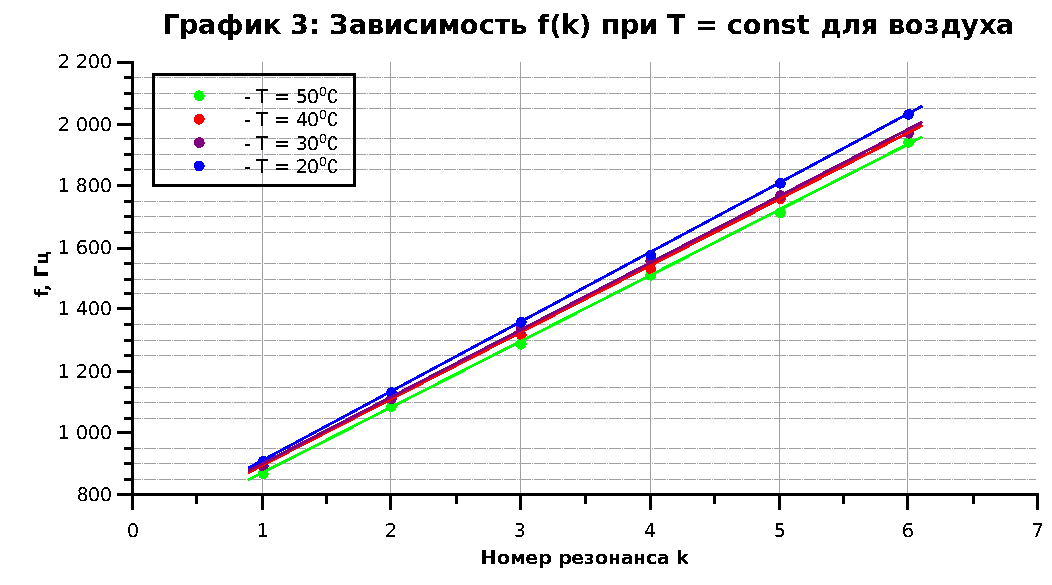
\includegraphics[scale=0.65]{Graph3.pdf}
\end{figure}
	\newpage
	Вычислим с помощью полученных графиков скорость звука в воздухе и рассчитаем погрешности.

	Длина трубы постоянная и равна $$L = 800 \pm 1 \: мм$$

	Погрешность $\sigma_{c}$ отдельного измерения определяется следующей формулой:
	$$ \sigma_{c} =c \sqrt{\Big(\frac{\sigma_{L}}{L}\Big)^2+ \Big(\frac{\sigma_{A}}{A}\Big)^2},$$
	где $A$ - коэффициент наклона прямой на графике.

	Результаты представлены в таблице 5:


\begin{table}[h!]
\centering
\begin{tabular}{|c|c|l|c|l|}
\multicolumn{5}{c}{\textbf{Таблица 5}}                                                                                               \\ \hline
\textbf{T, $^{\circ}$C} & \textbf{T, K} & \multicolumn{1}{c|}{\textbf{f, Гц}} & \textbf{с, м/c} & \multicolumn{1}{c|}{\textbf{$\gamma$}} \\ \hline
50                     & 323           & 212,7                               & 340,32          & 1,251                                  \\ \hline
40                     & 313           & 215,3                               & 344,48          & 1,322                                  \\ \hline
30                     & 303           & 216,4                               & 346,24          & 1,380                                  \\ \hline
20                     & 293           & 224,5                               & 359,2           & 1,536                                  \\ \hline
\end{tabular}

\end{table}


	По полученным данным расчитаем $\gamma$.
	$$\overline{\gamma} = 1,372$$
	$$\gamma_{сл} = \sqrt{\frac{\sum_{i=1}^{4} (\gamma_{i}-\overline{\gamma})^2}{3}} = 0.04 .$$
	Косвенная погрешность определения $\gamma$ мала, так как $\frac{2\sigma_c}{4c} \approx 0,25 \%.$
	Итак, $$\gamma = 1,37 \pm 0,04 ,$$ что в пределах погрешности совпадает  с теоретическим значением $\gamma = 1,4 .$
	
\section*{Вывод}
Мы измерили показатель адиабаты использовав скорость звука при помощи резонансных пиков зависимости амплитуды принимаемого сигнала при прохождении в закрытом пространстве от расстояния, проходимого звуком в одну сторону из-за появления стоячих волн, результаты эксперимента совпали с табличными значениями. $\gamma = 1,37 \pm 0,04$.

Также измерили скорость звука для воздуха и для углекислого газа. Экспериментальные данные с хорошей точностью совпали: для воздуха: $c = \left(3,5 \pm 0,3\right) \times 10^{2} \; \frac{м}{с},\\\text{для CO2: } c = \left(2,8 \pm 0,3\right) \times 10^{2} \; \frac{м}{с}.$

\end{enumerate}

\end{document}